\documentclass[10pt,conference,compsocconf,letterpaper]{IEEEtran}

\makeatletter
\def\ps@headings{%
\def\@oddhead{\mbox{}\scriptsize\rightmark \hfil \thepage}%
\def\@evenhead{\scriptsize\thepage \hfil \leftmark\mbox{}}%
\def\@oddfoot{}%
\def\@evenfoot{}}
\makeatother

\pagestyle{headings}
\usepackage{graphicx}
\usepackage[noadjust]{cite}
\usepackage{tabularx}
\usepackage{times}
\usepackage{alltt}
\usepackage{verbatim}
\usepackage{moreverb}
\usepackage{amsmath}
\usepackage{amssymb}
\ifCLASSINFOpdf \else \fi
\usepackage{url}
\usepackage{epsfig}
\usepackage{subfigure}
\usepackage{multirow}
%\usepackage{slashbox}
\usepackage[ruled,vlined]{algorithm2e}
\usepackage{mathrsfs}
\usepackage{amsthm}

\usepackage{dsfont}
\usepackage{cases}

\newtheorem{theorem}{Theorem}
\newtheorem{definition}{Definition}
\newtheorem{Lemma}{Lemma}

\newcommand{\ie}{{\em i.e.}}
\newcommand{\eg}{{\em e.g.}}
\newcommand{\et}{{\em et al.}}
\newcommand{\st}{{\em s.t.}}

\begin{document}

\title{Quality Evaluation of Crowdsensed Fingerprints for Indoor Localization}

%
%\author{\IEEEauthorblockN{Mei Wang$^1$, Xiaohua Tian$^{2,3}$, Xinbing Wang$^{1,3}$}
%\IEEEauthorblockA{
%1. School of Electronic, Info. \& Electrical Engineering, Shanghai Jiao Tong University, China\\
%2. Dept. of Electronic Engineering, Shanghai Jiao Tong University, China\\
%3. National Mobile Communications Research Laboratory, Southeast University, China}
% \{mary1994, xtian, xwang8\}@sjtu.edu.cn}
%

\maketitle



\begin{abstract}

\end{abstract}


\section{Introduction}\label{sectionintro}
The past decade has witnessed a flourishing of indoor localization systems based on wireless techniques \cite{ rsscsi}, where the fingerprinting based methodology has been widely adopted due to its convenient deployability \cite{ mobicom04, horus }. The fingerprinting based indoor localization system has two phases: In the offline phase, the site surveyor observes the received signal strength (RSS) of Wi-Fi access points (APs) termed as RSS fingerprints at each reference point, and submit the fingerprints and the location information of the reference point to the localization database; in the online phase, a user needs localization service could submit the observed fingerprints to the database, which then returns the location of the reference point that matches the fingerprints best as the estimated location of the user.   

The fingerprinting based method utilizes Wi-Fi APs widely existing in buildings and has no need for other dedicated infrastructure; however, the site survey in the offline phase requires substantial efforts, which is hardly accomplished by any single entity. The recent advances of fingerprinting localization systems utilize mobile crowdsensing approach to collect fingerprints \cite{ wen2015fundamental, Chenshu14, luo2014piloc, shen2013walkie, ez10, Chintalapudi10}. Mobile crowdsensing is a cost-effective approach to collect large scale data for mobile applications, where individuals with hand-held mobile devices collectively contribute sensing data so that information of certain events could be retrieved \cite{crowdsensing, postedpricing}. Although sensing participants could receive certain rewards for the efforts and resources spent on the sensing activity, the cost of mobile crowdsensing is still much lower than deploying the dedicated sensing networks \cite{ crowdsensing}. 


As the crowdsensing data are collected by unprofessional participants with non-dedicated equipment, the sensing data obtained are usually with considerable noise. The quality of the sensing data is the crux for evaluating contribution of the participants, which is the vitally important for effective utilizing rewards to incentivize participants to accomplish sensing tasks satisfactorily. However, how to evaluate the quality of the crowdsensing data is a challenging issue, because there is no ground truth for the collected data to be compared with. Efforts have been made to evaluate the crowdsensing data quality \cite{ Crowdloc14}, and the task allocation scheme \cite{ Taskselection15, recruit}. and incentive mechanisms considering the data quality are proposed. 

While the efforts have been made for quality-driven incentive mechanism\cite{Lbs2, noise,Pengdan15, incentive, Incentive2}, the state of the art method for crowdsensing data collection still focus on the incentive of workers. The economical problem is considered in \cite{Pengdan15}, however, the budget of the platform and is not included. Besides, all the work listed above do not consider the situation when data is coming in a sequential order and only 
available in each round. How to acquire the high-quality data that is in a sequential order given the limited budget is still not fully investigated, which is the focus of this work. Our motivation is two-fold. On one hand, the existing work for sequential data procurement in the literature \cite{abernethy2015low}do not work well for the situation of indoor localization; on the other hand, we want to build a concrete measurement of RSS data specifically for the active learning mechanism. Our contributions are as following.

First, we design an effective way to measure the quality of RSS data. [To be completed by WenXin] With such a measurenent, we successfully convert the problem into the basic framework of how to acquire the RSS data of best quality with the lowest costs.

Second, we produce a mechanism for RSS data procurement under a relatively nicer assumption that the costs of data are drawn according to a known distribution. Based on this assumption, the performance of our mechanism is dependent on both the quality of prior knowledge about the distribution of the costs and the regularity of the data. When the costs of data is relevant to a distribution that we know well the mechanism can perform well. 

Third, we generalize the mechanism to a more general case where the incoming cost of data is adversarially given. \emph{Using the technique of varitional calculus, we give an upper regret bound.](do not know whether this should remain} The mechanism is robust in most indoor-localization situations, even the prior knowledge of the costs is not well understood and the noise in the crowdsensing data is rather arbitrary. And we further provide a most economical data procure mechanism when the accuracy of RSS data is required.

The remaining of the paper is organized as following. The system structure and settings are given in section \ref{sysmodel}. The measurement  RSS data quality is presented in Section \ref{loss}. Section\ref{probdef}  gives the abstract definition for the online data procurement mechanism. Section \ref{weaksolution} describes the mechanism under the simple assumption that the costs data are drawn in a distribution. Section \ref{mainsolution} presents a generalized and more robust mechanism for the RSS data procurement. Section \ref{exp&sim} gives our simulations and experiments for the mechanism we given before.



\section{Related Work \label{sectionrelatedwork}}
\subsection{Crowdsensing for Indoor Localization}

The industrial context our work pertains to is fingerprinting localization based on mobile crowdsensing. In regard to localization via fingerprints, Kaemarungsi and Krishnamurthy draft out the analytical model of it \cite{kaemarungsi2004modeling}, and Wen \emph{et al.} \cite{}further dig into this model combined with received signal strength, making out theoretical analysis of its limits on indoor localization \cite{wen2015fundamental}. Concerning mobile crowdsensing, Ganti \emph{et al.} presents a brief overview of concrete applications about this technique, dissects its distinctive useful features and furthurmore blueprints its future utilization and challenges\cite{ganti2011mobile}.Meanwhile, mobile crowdsensing approach has been applied to various domains such as transportation \cite{transportation2}, environment surveillance \cite{environment,environment2} and location based service \cite{lbs, lbs2},evincing the research value of this method in reality.

\subsection{Online Learning and Online Optimization}

One basic theory that our work based is online learning, which is applied to the fingerprinting data procurement phase of indoor localization. Zinkevich provided an introduction of online convex programming and an effective algorithm: Generalized Infinitesimal Gradient Ascent for this problem, making for the fundamental construction of online learning\cite{zinkevich2003online}.
Online convex optimizing theory has been comprehensively displayed in \cite{shalev2011online}, on which our onlihne learning researches are predicated. However, it only derives a general model aiming at online convex optimization, without considering the economical problem and can not be appplied in many practical situations, especially when the access of all the data is expensive. 

One of the kernel issues in online learning is how to evaluate the quality of data acquired. In online learning, an acknowledged way to assessing procured data is the regret, which can be viewed informally as the difference of overall loss between the strategy one chooses and the theoretical best strategy reaching the least loss \cite{shalev2011online}.Abernethy \emph{et al.} crystallize a particular online problem setting with a regret analysis attached\cite{abernethy2015low}. 

\subsection{Our particular problem}

Based on the theoretical tool mentioned above, Our particular problem can be interpreted as: minimizing the overall regret in online learning with a fixed upper limit of budget.With regard to this problem setting, Abernethy \emph{et al.} presented an all-round dissection of it\cite{abernethy2015low}. They firstly utilized the classical online learning algorithm: Follow the Regularized Leader(FTRL) to update steadily the hypothesis in every round the mechanism should give, in light of information the mechanism has acquired in previous rounds about offered hypotheses and suffered loss. Then They embedded FTRL in their main algorithm: Mechanism for no-regret data-purchasing problem, which resolved the problem with an upper regret bound $O(T/\sqrt{B})$. Compared with what Abernethy \emph{et al.} have done\cite{abernethy2015low}, what is special in our work is to further lower the regret bound of online learning in the context of indoor localization--a brand new research background in online learning realm.\\
\indent In terms of concrete techniques applied in this particular problem, importance weighting is an important one, playing a crucial role in estimating unbiasedly the cumulative loss suffered until the current round\cite{abernethy2015low}. This technique is also a research point in our work, and we focus on providing an alternative form of the unbiased estimator to reach better regret bound. One specific application of importance weighting methods--binary classification is shown and analyzed in \cite{beygelzimer2009importance}.\\
\indent Moreover, a bottleneck in solving this particular problem is the complex form of our objective function and budget constraint, with unknown distributions of costs in each round and an inequality containing integral. Abernethy \emph{et al.} rendered a more computable convex optimizing problem\cite{abernethy2015low} under an easier form and generalize the result to  main setting. However, this method can only derive an approximated solution and the corresponding bound may not be tight enough. In our work we try to get access to the accurate solution of this problem, by means of calculus variation. The applicability and methods of calculus variation are illustrated in detail in \cite{liberzon2012calculus}  . A concrete example taking advantage of it lies in \cite{roth2012conducting},which dealt with the problem that minimizing the variance of estimator with a given price distribution and a fixed budget by calculus variation. Nevertheless, it concentrated on the offline situation, deviating from our online background.

\section{System Model}\label{sysmodel}
In this section we describe our system model and give out the problem formulation.

As shown in Figure~\ref{}, we present a mobile crowdsensing system consisted of \emph{Data Purchaser}, \emph{Trading Platform} and several \emph{Workers}. For the purpose of performing accurate indoor localization in region $\mathcal{V}$, the data purchaser has to build the corresponding \emph{Fingerprint Database} of \emph{Received Signal Strength}(RSS). Therefore the data purchaser releases tasks of collecting data--RSS value on the platform. For a specific location $s\in \mathcal{V}$, we use $\mathds{W}_s=\{w_1,w_2,...,w_{N_s}\}$ to denote the corresponding applicants set. To simplify the notation, we omit the identification of $s$ in almost all the rest of this paper. Without loss of generality, we mainly focus on workers with the same location's data. It's rational that data purchaser need to buy several data points at one location since the RSS value is not constant, in fact it obeys some probability distribution, we assume that its probability density function is $\mathcal{D}(\cdot)$. Consequently, we need several amounts of samples to learn the distribution, more specifically, to estimate the mean value of RSS.

At the very beginning, the data purchaser needs to submit his \emph{Pricing Mechanism} $\mathbb{M}$ to the platform. Here we consider the most nature trading scenario: these $N$ workers arrive in a sequential way with his data $x_i$. Once agents $i$ arrives, he submit his bid $c_i$ to the platform and the platform compute its price $p_i$ using a mechanism $\mathbb{M}$. If $p_i\geq b_i$ then agents $w_i$ accept this transaction: the platform pays $b_i$ to worker $i$ and receives data $x_i$, otherwise the worker reject the transaction and the platform receives null signal.

\begin{table}[h]
\caption{\textsc{Notations}} \label{tab:Notation}
\centering
\resizebox{\columnwidth}{!}{
\begin{tabular}[t]{l|p{7cm}}
\hline
Notation&Remark \\
\hline\hline
$\mathcal{V}$ & Indoor location region\\
$s$ & A specific location\\
$\mathds{W}_{s}=\{w_1, \cdots,w_{N_s}\}$ & Applications set for location $s$\\
$\mathcal{D}(\cdot)$ & Probability density function\\
$\mathbb{M}$ & Pricing mechanism\\
$w_i$ & The $i_{th}$ worker\\
$x_i, b_i, p_i$ & $w_i$'s data, bid, and corresponding price\\
\hline
\end{tabular}
}
\end{table}

\section{Analysis of two-dimensiion localization}\label{loss}
\subsection{One-Time Measurement for Single AP in Two-Dimension Space}
Hereinafter we are devoted to the analysis of one-time measurement for a single AP in two-dimension physical space. Although our research object has been upgraded from a corridor to a room, a more complex one, the kernel thought of our analysis is analogical to that in one-dimension condition, with solely difference in addressing the problem of physical space in a two-dimension Cartesian Coordinate. Ultimately we derive the expression of $P_{high}$ and $P_{low}$ in the sample space of two-dimension physical space, which form $[{P_{low}},{P_{high}}]$, as the feasible interval for judging a users' location, and furthermore study the possible localizing error incurred by imperfect data.

\subsubsection{Maximum Likelihood Estimation in two-dimension physical space}
\begin{figure}[!htbp]
\centering
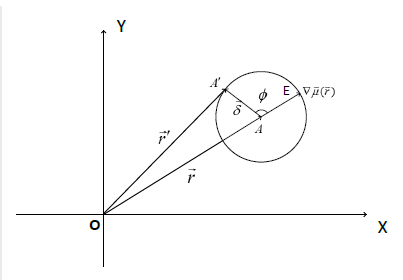
\includegraphics [width = 7cm]{Figure1.png}
%\vspace{-2 mm}
\caption{Description.}
\label{fig:1}
%\vspace{-5 mm}
\end{figure}

Figure 1 illustrates our model in two-dimension physical space. We designate the AP we sample as the original point $O$ of the coordinate system, and denote $A$ as as the users' actual location which we focus on estimating. Assume that the distribution of RSS around $A$ are circular symmetric , therefore we can define region $E$ as a circle with radius $\delta$, and measurement in it means that the user is estimated at $A$ while outside it indicates at other possible locations rather than $A$. Note that if we consider any one of the straight lines through $A$, then the distribution and localization are identical to those in one-dimension situation. Then we define the vector from $O$ to $A$ in physical space as $\vec r$ and to any location $A'$ on the boundary of $E$ as $\vec r'$. Therefore, $\vec \delta  = \vec r' - \vec r$ in Figure 1 can be clearly deemed as the difference between user's real location and our estimation result, \ie, the accuracy of our localization. In addition, since $O$ is the AP we consider, the gradient of RSS at $A$ (\ie, $\nabla \vec \mu (\vec r)$ in Figure 1) must be the same direction as $\overrightarrow{OA}$. We also define $\varphi$ as the inserted angle between $\vec \delta $ and $\nabla \vec \mu (\vec r)$, $\varphi  \in \left( { - \pi ,\pi } \right]$, where $\varphi < 0$ denotes the absolute value of $\varphi$ is less than $\pi$ clockwise (\ie, starting from $\nabla \vec \mu (\vec r)$ to $\vec \delta $ while $\varphi  > 0$ indicates the opposite.

Similar as one-dimension condition, MLE can be the judgment of whether a user is located at $A$ in two-dimension physical space based on our localization system. For single-measurement situation the MLE can be expressed as:
\begin{align}
{f_{\vec r}}(P) \ge {f_{\vec r + \vec \delta }}(P),
\end{align}
where ${f_{\vec r}}(P)$ denotes the probability distribution function of RSS pertaining to the access point $P$ at location $\vec r$. However, unlike in one-dimension condition $\vec \delta$ is reduced to a scalar $\delta$ without directions ($\varphi$) taken into consideration, two-dimension problem requires MLE satisfy every single direction mapped by every possible value of $\varphi  \in \left( { - \pi ,\pi } \right]$. Hence, $\varphi$ should be embedded in our analysis.

In order to render our explanation simpler and clearer, we rotate the coordinate system to a point where the new x-axis covers $\overrightarrow{OA}$ (Figure 2). Meanwhile $\nabla \vec \mu (\vec r)$ is also co-linear with the x-axis. Then aiming to derive the specific expression of MLE, we firstly make some assumptions:
\begin{itemize}
\item[(1)] The radius value $\delta$ should be small enough since we intend to meet high localizing accuracy (distinguishing different locations with very short distances from each other). Therefore, $E$ can be viewed as a very small region in physical space.
\item[(2)] $\left| {\nabla \vec \mu (\vec r)} \right|$ equals to the difference between $\mu (\vec r + \vec \delta )$ and $\mu (\vec r)$ in which $\vec \delta $ is co-linear with the new x-axis. Hereinafter in this section we denote $\nabla$ as $\left| {\nabla \vec \mu (\vec r)} \right|$ to simplify the mathematical expression.
\item[(3)] Every line perpendicular to $\nabla \vec \mu (\vec r)$ represents that all locations on this line inside $E$ have uniform RSS value. Factually according to the direct correlation between distance and RSS, the equi-value delineation of RSS should be a circle rather than a straight line. Nevertheless, due to the fact that $E$ is small enough, the equi-value curve inside $E$ can be approximated as a line segment.
\item[(4)] The distribution of RSS strength in two-dimension physical space should be a two-dimension normal distribution. However given that every line vertical to the new x-axis represents an identical RSS value for all locations on it, the normal distribution is degraded to one dimension if we consider the distribution on the new x-axis.
\end{itemize}

It is clear that the RSS value of $\vec r$ (\ie, $\mu (\vec r)$) corresponds the largest measuring probability when $\vec r$ is which we aim to locate. \textbf{Original Graph in Section 4.1}. Hence we can derive
\begin{align}
{f_{\vec r}}(P) = \frac{1}{{\sqrt {2\pi } \sigma }}{e^{ - \frac{{{{(x - \mu (\vec r))}^2}}}{{2{\sigma ^2}}}}},
\end{align}
where $\sigma$ represents the intrinsic noise. Combining with Assumption 3 and 4, we can further derive ${f_{\vec r + \vec \delta }}(P)$ predicated on the representative condition in Figure 2.
\begin{align}
{f_{\vec r + \vec \delta }}(P) = \frac{1}{{\sqrt {2\pi } \sigma }}{e^{ - \frac{{{{(x - (\mu (\vec r) + \nabla \cos \varphi ))}^2}}}{{2{\sigma ^2}}}}}
\end{align}
Then to meet the conditions of MLE, we have:
\begin{align}
\frac{1}{{\sqrt {2\pi } \sigma }}{e^{ - \frac{{{{(x - \mu (\vec r))}^2}}}{{2{\sigma ^2}}}}} \ge \frac{1}{{\sqrt {2\pi } \sigma }}{e^{ - \frac{{{{(x - (\mu (\vec r) + \nabla \cos \varphi ))}^2}}}{{2{\sigma ^2}}}}}
\end{align}
for all $\varphi  \in \left( { - \pi ,\pi } \right]$. Simplify it we will have:
\begin{align}
{(x - \mu (\vec r))^2} \ge {(x - (\mu (\vec r) + \nabla \cos \varphi ))^2}
\end{align}
In order to gain clearer insight into this inequality, Figure 3 is displayed as follows in which the sample space is concerned.

In Figure 3, the endpoints of this line segment represent the extreme conditions that $\varphi$ equals to 0 and $\pi$. Analogical to one-dimension analysis, we can derive
\begin{align}
{P_{high}} = \frac{{\mu (\vec r) + (\mu (\vec r) + \nabla \cos \varphi )}}{2} = \mu (\vec r) + \frac{{\nabla \cos \varphi }}{2}\\
{P_{low}} = \frac{{\mu (\vec r) + (\mu (\vec r) - \nabla \cos \varphi )}}{2} = \mu (\vec r) - \frac{{\nabla \cos \varphi }}{2}
\end{align}
which evinces that our localizing estimation will be judged to $A$ if and only if $P$ satisfies ${P_{low}} \le P \le {P_{high}}$. Here we limit $\varphi  \in [ - \frac{\pi }{2},\frac{\pi }{2}]$ to ensure ${P_{high}} \ge {P_{low}}$, if $\varphi  \notin [ - \frac{\pi }{2},\frac{\pi }{2}]$ then we can exchange the expression of ${P_{high}}$ and ${P_{low}}$ to maintain ${P_{high}} \ge {P_{low}}$. \textbf{---Rule 1)} Since the \textbf{equality(n)} holds for any $\varphi  \in \left( { - \pi ,\pi } \right]$, thus if fall into all possible intervals $[{P_{low}},{P_{high}}]$ then it will be classified into location $A$. The extreme condition is that while $\varphi  = \frac{\pi }{2}$, ${P_{high}} = {P_{low}}$, indicating that $P$ will be judged to $A$ if and only if $P = {P_{high}} = {P_{low}}$. That is to say our measurement must estimate the user��s location exactly at $r$, the real location. However, as error exists all the time in measurement and estimation, it is practically impossible to reach this extreme condition. Since that our previous analysis cannot be directly applied to realistic problems.

\begin{figure}[!htbp]
\centering
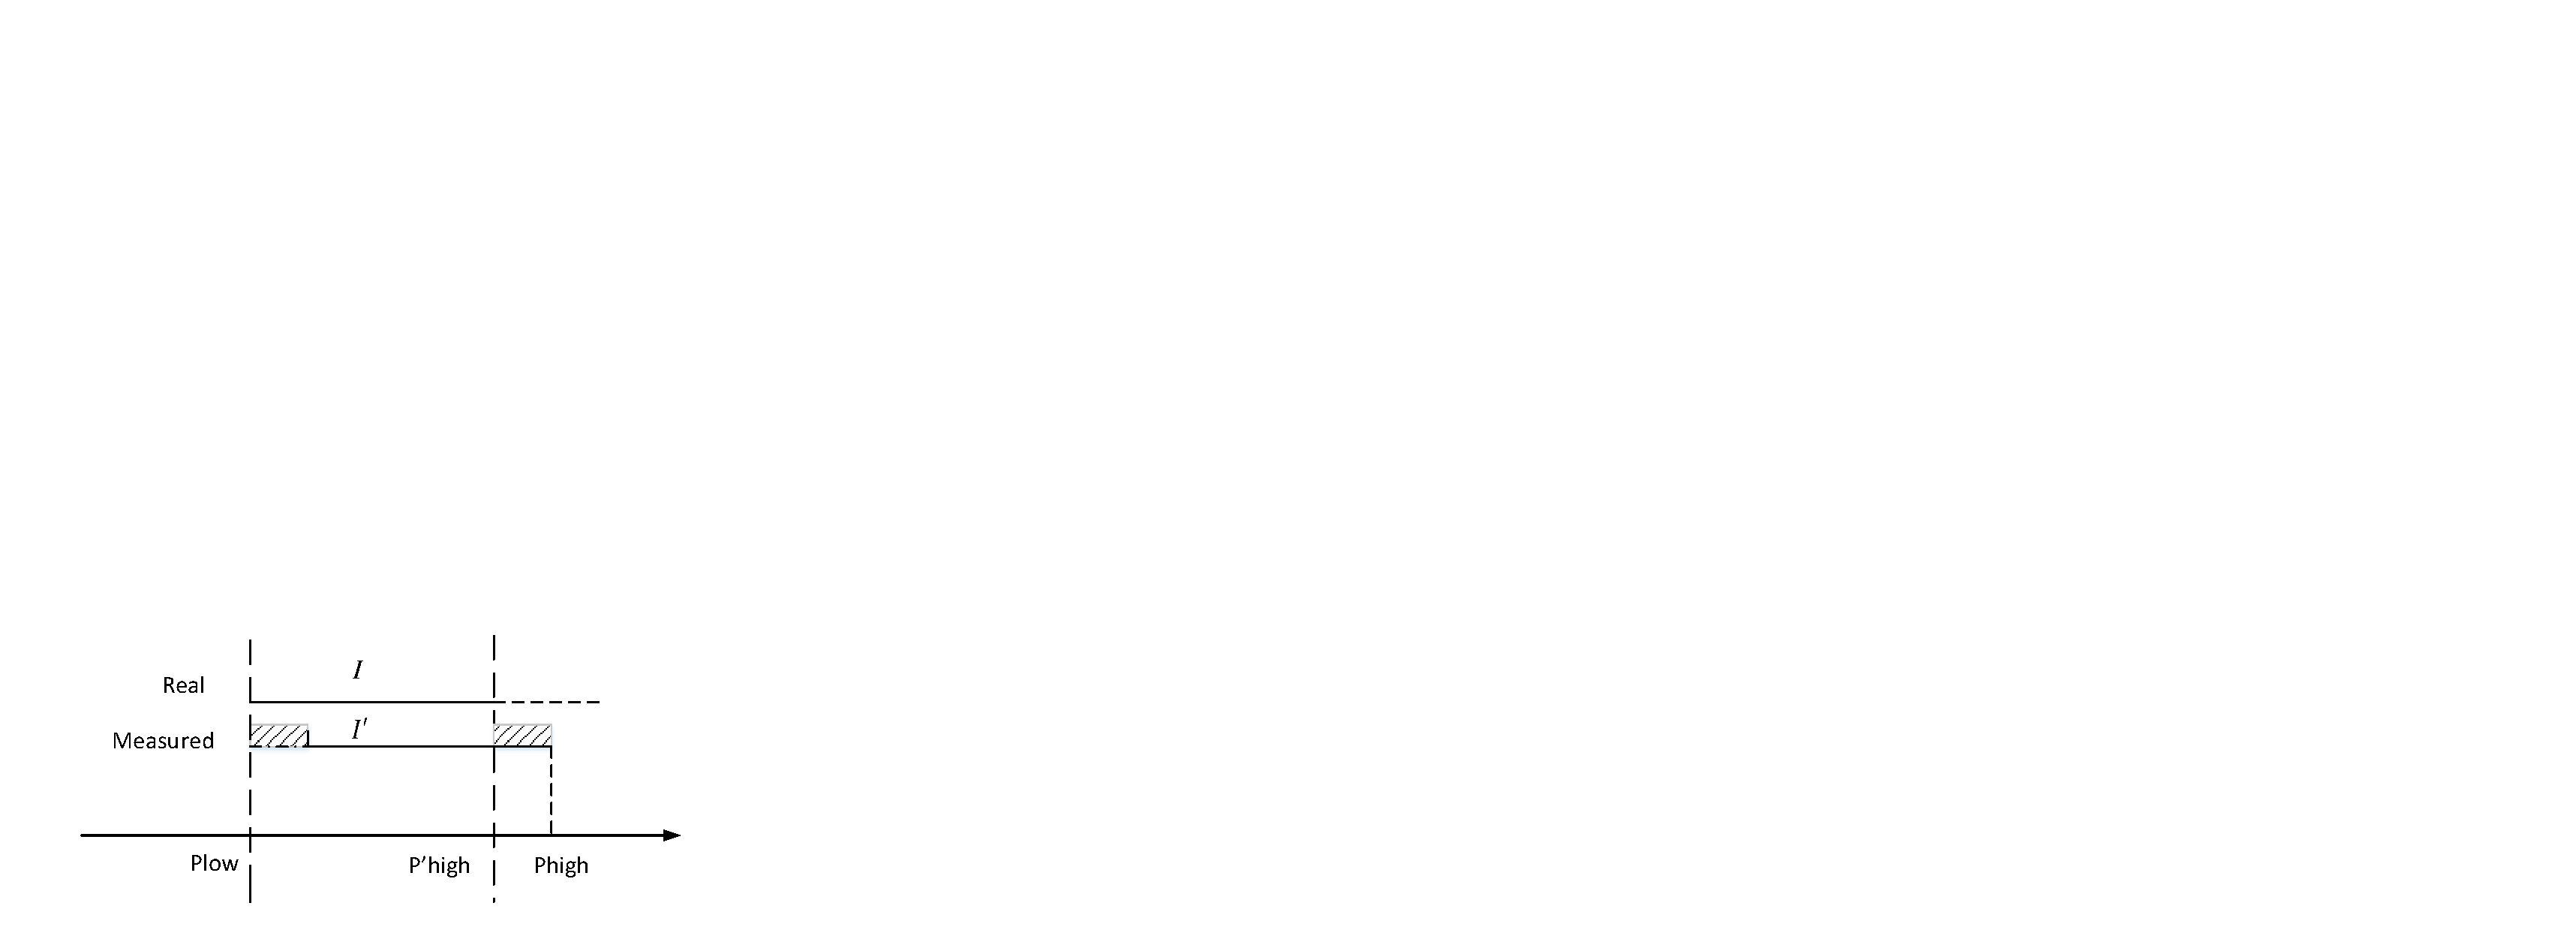
\includegraphics [width = 7cm]{Figure4.pdf}
%\vspace{-2 mm}
\caption{Description.}
\label{fig:4}
%\vspace{-5 mm}
\end{figure}

However, noticing that practical indoor localization divides a room into many small square blocks and denotes the center of each block as a possible estimated location (\ie, if an estimation falls into one of these blocks, then the location we determine this user is the center of this block.) Therefore, it is not necessarily for us to consider all locations on the boundary of $E$ as analysis above. Instead we may solely concentrate on four blocks adjacent to our target block ($A$ is the center), and denote each center of these four block as $B, C, D, E,$ displayed in Figure 4. Under this circumstances, we will only have to meet four MLE constraints which relax our feasible solution from a single point $P$ to an interval. We will discuss it in detail with Figure 5.

Figure 5 is similar to Figure 3 and we define parameters in accordance with Figure 4. Then based on previous analysis we can easily write the simplified MLE constraints of $B, C, D, E$:
\begin{align}
\left\{\begin{array}{l}
{(x - \mu (\vec r))^2} \ge {(x - (\mu (\vec r) + \nabla \cos \phi ))^2}\\
{(x - \mu (\vec r))^2} \ge {(x - (\mu (\vec r) + \nabla \sin \phi ))^2}\\
{(x - \mu (\vec r))^2} \ge {(x - (\mu (\vec r) - \nabla \cos \phi ))^2}\\
{(x - \mu (\vec r))^2} \ge {(x - (\mu (\vec r) - \nabla \sin \phi ))^2}
\end{array}\right.
\end{align}
Therefore we can draw out Figure 6 in light of Figure 3. Then according to above analysis, it is clear that we can derive the feasible interval as
%\begin{equation}
%\begin{split}
%&I = [ {\mu (\vec r) - \frac{{\nabla \min \left\{ {\cos \phi ,\sin \phi } \right\}}}{2},\mu (\vec r)+\\ &\frac{{\nabla \min \left\{ {\cos \phi ,\sin \phi } \right\}}}{2}} ]
%\end{split}
%\end{equation}
\begin{equation}
\begin{split}
&I =\\ 
&\left[ {\mu (\vec r) - \frac{{\nabla \min \left\{ {\cos \phi ,\sin \phi } \right\}}}{2},
\mu (\vec r)+\frac{{\nabla \min \left\{ {\cos \phi ,\sin \phi } \right\}}}{2}} \right]
 \end{split}
 \end{equation} 
where $\phi  \in \left[ { - \frac{\pi }{2},\frac{\pi }{2}} \right]$ and follows Rule 1. It demonstrates that a user is measured in block $A$ if and only if the estimation of him falls into $I$. Thus the reliability of our one-time measurement analysis of two-dimension physical space can be interpreted as:
\begin{align}
\begin{split}
R &= \int_{{P_{low}}}^{{P_{high}}} {{f_r}(P)dP }\\
 &=\int_{\mu (\vec r) - \frac{{\nabla \min \left\{ {\cos \phi ,\sin \phi } \right\}}}{2}}^{\mu (\vec r) + \frac{{\nabla \min \left\{ {\cos \phi ,\sin \phi } \right\}}}{2}} {\frac{1}{{\sqrt {2\pi } \sigma }}{e^{ - \frac{{{{(x - \mu (\vec r))}^2}}}{{2{\sigma ^2}}}}}dx}
 \end{split}
\end{align}

\subsubsection{Imperfect Data}
Then we extend our study to the influence of imperfect data in a two-dimension physical space. Recall in one-dimension analysis the imperfectness of received data is described as a deviation of line segment in the sample space. Therefore although our physical space has upgraded to two dimension, our sample space is still in one dimension as given above and what we receive are data of RSS, reflected directly in sample space. Thus we can imitate the method to derive error analysis similar as that of one-dimension situation.

We still set our target region as  and consider $A$ abut to $B, C, D, E$ abut to $A$. Firstly it is reasonable to assume that the probability that a user is located at any location in $A$ to be identical, so the distribution of user's true location in  is a uniform one, whose probability distribution function is:
\begin{align}
p{f_A}(Q) = \left\{ \begin{array}{l}
\frac{1}{S},\quad Q \in A\\
0,\quad Q \notin A
\end{array} \right.
\end{align}
where $A$ denotes the target region, $S$ represents its area and $Q$ means a user's true location. Note that every $Q$ in two-dimension physical space can be mapped to the one-dimension sample space according to Assumption 3. Now we set the user's true location in physical space is ${Q_0}$ and its corresponding point in sample space is $X_0$. Figure 7 illustrates the influence of imperfectness of data procured, which results in the deviation of feasible interval $I$ in sample space from its true range. As in Figure 7 we denote the right endpoint of true range as $X_1$ and deviated range as $X_2$, hence we can discover if a point $X_0$  falls into interval $(X_1,X_2)$, then it will be falsely estimated: $X_0$ should have been classified into region $B$ while because of the deviation it is determined to be in region $A$. The same goes for the left side of region $A$, the boundary point of $A$ and $C$. Given our situation, then we can derive the probability of localizing error as:
\begin{align}
P(err) &= \iint_A {{f_A}}(Q)P(err|X = {X_0})dxdy\\
&= 2\iint_A {{f_A}}(Q)\int_{{X_1}}^{{X_2}} {\frac{1}{{\sqrt {2\pi } \sigma }}{e^{ - \frac{{{{(X - {X_0})}^2}}}{{2{\sigma ^2}}}}}} dXdxdy
\end{align}

\section{Low-cost data purchasing problem}\label{probdef}
In this section, we will abstractly define the problem of the designing of the effective mechanism to acquire the RSS information collected by the crowds. 

\subsection{Preliminaries}
We first give the concept of loss and regret. The loss function that reflects the data quality is defined in the space $H\times Z\to R$, where $H$ is the hypothesis class and $Z$ is the space of the objects. We expect the loss function to get its minimum value when the data is exactly the ideal data. In our setting, the hypothesis $h$ is the mean value and variance of RSS fingerprinting data, and the hypothesis class $H$ is our expected internal of mean value and  variance. 
\begin{equation}
f_t(h_t)=
\end{equation}
 After we acquire the loss function, we give the concept of the regret function.
\begin{equation}
R(T)=\sum_{t=1}^Tf_t(h_t)-\min_{h^*\in H}\sum_{t=1}^Tf_t(h^*_t)
\end{equation}
where $h^*$ is the optimal choice, causing the least loss in our solution space $H$. The regret function reflexes how the data deviate from the desired value, the real mean and variance of RSS. We also make some assumptions for this problem
\begin{enumerate}
\item the agents may lie about the cost
\item 
\item the cost of each data  lies in an internal between  0 and $M$
\end{enumerate}


\subsection{Online Learning Algorithms}
Online learning is a widely used learning paradign. The goal of online learning is to produce the best hypothesis when data is in sequential order
We here use the classical Online Gradient Descent(OGD) algorithm to work as the Online Algorithms. It has been proved that the OGD has an upper bound of regret of $O(\sqrt{T})$, which ensures that the average regret tends to zero when $T$ goes to infinite. There are also many kinds of other Online Algorithms which can be found in \ref{OLServey}, etc. The OGD is described as following. In each time $t$, the algorithm choose the smallest hypothesis in $H$ such that the sum of the loss function plus a regularizer $R$ get its infimum
\begin{equation}
h_t=arg\min_{h\in H}\sum_{i=1}^{t-1}f_i(w)+R(w)
\end{equation}.



\subsection{Importance Weighting technique}

In tradational online learning problem, all the data will be used to produce the total regret. In our low-cost purchasing problem, the mechanism do not get access to data and obtain a loss in each time $t$.  the estimation of loss is $E(\sum_{t=0}^T\delta_t f_t)=\sum_{t=0}^T q_t f_t$, where $\delta_t$ is the function showing whether the data is procured. However, the definition of regret still includes all the loss, whether it has been used or not.  In order to get an unbiased estimator, we define
\begin{numcases}{\hat{f_t}(h)=}
  \frac{f_t(h_t)}{q_t} & if the is  \\
  0 & else 
\end{numcases}
.
\subsection{Problem definition}
We consider that the data collected through crowdsensing coming in a sequence of $d_1,,,d_T$, with each of them contains a cost $c_1,,,c_T$. We should design a mechanism that can choose whether we should buy the data or not. However, we have no means to know either the quality of data is good enough for localization or there will be a better one coming in the sequence. Under the framework of online machine learning, we formally define our mechanism as following
\begin{definition}{}\label{def:1}
Given a sequence of data ${d_1,,,d_T}$ coming in time $1,,,,,T$ with each data possessing a posted price $c_t$, $c_t\in [0,M]$. 
\begin{enumerate}
\item The mecahnism post a hypthesis $h_t$ from OLA
\item The mechanism post a price $p_t$ according to a probablity distribution function $g_t(p_t)$.
\item If the $p_t>c_t$ agent accepted the price, the mechanism send the loss function $f(h_t)/q_t$ back to the OLA and pay for the posted price $p_t$. If $p_t<c_t$the agent rejected the price, the mechanism send a null data to the OLA . 
\end{enumerate}
The mechanism outputs a hypothesis $\overline{h}\in H$
\end{definition}
And clearly, our kernel problem is to find the best distribution used for the mechanism to post its price 
\subsection{online batch to conversion}
The meachanism and online learning algorithm produces a sequence of hypothesis $h_1,,,h_T$. The main goal of our algorithm is to get the best hypothesis $\overline{h}$, the mean value and variance of RSS, from the sequence. One simple aproach is to average every hypothesis $h_t$ acquired in each time $t$.
\begin{equation}
\overline{h}=\sum_{t=1}^n h_t
\end{equation}
It has been proved that 

\section{The main setting: regret minimization senario}\label{mainsolution}
In this senario, the mechanism has a fixed budget. The main purpose of the mechanism is to get a high accuracy of localization informaiton, which is consistent with our definition of loss function and regret. 
\subsection{Estimate the upper bound of regret}
We will first find the upper bound of the regret. In normal case, the regret bound of OGD is 
\[\frac{||h||^2}{2\eta}+\eta \sum_{t=1}^T\nabla f_t(h_t)^2\]
, which is a well known result. Under the importance weighting framework, we give the regret bound in the following lemma
\begin{Lemma}{}
The regret bound produced by the mechanism in \ref{def:1} using the OLA of OGD is bounded by
\begin{equation}
R(h)=\frac{||h||^2}{2\eta}+\eta E(\sum_{t=1}^T\frac{\nabla f_t(h_t)^2}{q_t})
\end{equation}
\end{Lemma}
The $\Delta_{h_t,f_t}^2$ denotes the duality norm of $||\nabla f_t||$. The \ref{} is quite easy to be proved under our setting that the loss function $f_t$ is of strong convexity.

\subsection{Derivation of the Regeret Minimization Problem}

First consider the unconstrained problem. If $\overline{y}$ is the local minimum of the functional $J(y)$
if $y$ is the local niminum of $J(y)$, then it holds that $\forall \hat{y}$ in a function space $V$
\[\delta J|_y(\hat{y}-\overline{y})\geq 0\]
where $,\delta J|_y(\hat{y}-\overline{y})$is the Gateaux deravative of J in the direction of $\hat{y}-\overline{y}$. 

We then consider the constraint problem. For the constraint optimization problem, we have that if $y$ is the extremal of the constraint problem, then it is also the extremal of the augmented cost functional(Lagarangian) $J(y)+\lambda C(y)$,where the $\lambda$ is the Lagarange Multiplier, and $C(y)$ is the constraint.

We come back to our problem. We first give our function space $V=\{y|y(0)=0,y(M)=1\}$. And we denote our cost function as
\[M(F_1,,,F_n)= \sum_{i=1}^n \frac{\alpha_i}{1-F_i(c_i)}.\]
Then the augmented cost function is derived as
\[J(F_1,,,F_n,\lambda)=M(F_1,,,F_n)+\lambda( \sum_{i=1}^n\int_{c_i}^MxdF_i(x)-B) \]
According to the calculation, we obtain that for $\forall \hat{F}\in V$
\[\delta J|_{F_t}(\hat{F_t}-F_t)=\int_{c_t}^M(-\frac{\alpha_t}{(1-F_t(c_t))^2}+\lambda x)(\hat{f}(x)-f(x))dx\]
if $\overline{F}$ is the local minimum, then we have
\[\delta J(\hat{F_t}-\overline{F_t})\geq 0\]
holds for every $\hat{F}\in V$.Noticing that
\[\int_0^Mf_t(x)-f(x)dx=0\]
We must have 
\[-\frac{\alpha_t}{(1-F_t(c_t))^2}+\lambda x\geq 0\]
hold on every where on $[c_t,M]$
thus we obtain that
\begin{equation}
F_t(c)=\max\{1-\sqrt{\frac{\alpha_t}{\lambda c-\beta}},0\}\quad c\in(0,M) 
\end{equation}
Noticing that $F(x)$ is not continuous, according to Stieltjes Integral, we rewrite the constraint as following
\[ \sum_{i=1}^n(\int_{c_i}^Mxf_i(x)dx+(1-F_i(M)M)\leq B\]
The Stieltjes Integral here has its practical significance. Because we assume that the cost lies between $[0,M]$, in other word, the mechanism do not accept any price higher than $M$, thus for all posted price $c$ that are higher than $M$, the mechanism will only pay $M$ instead of $c$.
\subsection{Analysis of the result}
Now since we get the solution of the $F_t$, the remaining work is to determine the $\lambda$
. According to the property of Lagarangian, we have
\[\frac{\partial J}{\partial \lambda}=\sum_{i=1}^n(\int_{c_i}^Mxf_i(x)dx+(1-F_i(M)M)-B=0\]
After simple calculation, we can have an estimation of $\lambda$ as following
\begin{equation}
\sum_{t=1}^T\frac{\nabla f_t(h_t)}{\sqrt{\lambda}}({2\sqrt{M}-\sqrt{c_t})\leq B}
\end{equation}
Combining the result in \ref{}, we can have that when we set $\eta$ to $\sqrt{2T}$, we achieve the regret bound of approximate $O(\frac{T}{\sqrt{B}})$. One problem in this situation is that we may not get enough prior knowledge to both $c_t$ and $\nabla f_t$. One way to solve the problem is that we initially set $\sqrt{\lambda}$ to a very small value, e.g. $0.0001$.  Then in each time $t$, we update the value of $\sqrt{\lambda}$ with 
\[\sqrt{\lambda}=\sum_{i=1}^{t-1}\frac{\nabla f_t(h_t)}{t-1}(2\sqrt{M}-\sqrt{c_t}) \]


\section{The budget minimization senario}
In this senario, we consider the problem to find the most money-saving way to acquire the data inorder to achieve a satisfactory regret bound $R$. The objective function is in the form of a integral, which is not an easy problem of the classical optimization problem. Besides, to solve the very exact form of the budget . Thus we use the of the budget B as following
\begin{equation}
\sum_t c_t q_t \leq B \leq \sum_t Mq_t
\end{equation}
Thus what we have to do is to solve the optimization problem of the form
\begin{align}
&\min_{q_t} c_t\\
s.t. &\sum_t \frac{\nabla f_t^2}{q_t}\leq R\\
	&0\leq q_t \leq 1
\end{align}
\subsection{The optimal mechanism}
Consider the convexity of the objective function, we give the Lagrangian
\begin{equation}
L=\sum_t c_t q_t -\lambda(-\sum_t\frac{\nabla f_t^2}{q_t}+R-\sum_t\mu_t(1-q_t))
\end{equation}
The optimal K-T condition of the problem \ref{} is 
\begin{align}
\frac{\partial L}{\partial q_t}=c_t-\lambda[\frac{\nabla f_t^2}{q_t^2}]-\mu_i=0
\end{align}
when $q_t=1$, we get $u_i\neq 0$, when $q_t\neq 1$, $\mu_i=0$, thus we have
\begin{equation}\label{BC:q}
q_t=\min\{1,\sqrt{\frac{\lambda}{c_t}}\nabla f_t\}
\end{equation}
According to our constraint condition
\begin{equation}
\sum_t \sqrt{\frac{c_t}{\lambda}}\nabla f_t\leq R
\end{equation}
we can get an approximation of the $\sqrt{\lambda}$ through simple calculation
\begin{equation}
\sqrt{\lambda}=\frac{T}{R}\theta
\end{equation}
where we use $\theta$ to denote the term $\frac{1}{T}\sum_t\sqrt{c_t}\nabla f_t$.
Since \ref{BC:q} holds for $\forall c_t$, and $c_t$ is arbitrarily given.We may assume that the convoluted distribution function of the price mechanism is of the form 
\begin{equation}
F_t(c)=1-\sqrt{\frac{\lambda}{c}}\nabla f_t
\end{equation}
And the PDF is 
\begin{equation}
f(c)=\frac{1}{2}\sqrt{\frac{{\lambda}}{c^3}}\nabla f_t
\end{equation}
\subsection{result analysis}
Now we can make a relatively more precise estimate the budget $B$
\begin{align}
E(B)&=\sum_t\int_{c_t}^Mcf(c)dc\\
&=\frac{T^2}{R}\theta\varphi
\end{align}
where $\varphi=\sum_t\frac{1}{T}\nabla f_t(\sqrt{M}-\sqrt{c_t})$



\section{Experiments and Simulations}\label{exp&sim}
In this section, we give the ............ We use the data collected in FoxCom Shanghai,
\subsection{}

\section{Conclusion and Future Work}\label{concandfuture}


\bibliographystyle{IEEEtran}


%\bibliography{bibi}

\begin{thebibliography}{99}

\bibitem{rsscsi}
Z.~Yang, Z.~Zhou and Y.~Liu, ``From RSSI to CSI: Indoor localization via channel response,'' \emph{ACM Comput. Surv.}, vol.~46, no.~2, pp.1-32, 2013.

%related work part
\bibitem{kaemarungsi2004modeling}
K.Kaemarungsi, and P.Krishnamurthy, ``Modeling of indoor positioning systems based on location fingerprinting,'' in \emph{Twenty-third AnnualJoint Conference of the IEEE Computer and Communications Societies}, 2004, vol. 2, pp. 1012--1022.

\bibitem{wen2015fundamental}
Y.~Wen, X.~Tian, X.~Wang and S.~Lu, ``Fundamental limits of RSS fingerprinting based indoor localization,'' in \emph{Proc. IEEE INFOCOM}, 2015, pp.2479--2487.

\bibitem{ganti2011mobile}
R.K.Ganti, F.Ye, H,Lei, ``Mobile crowdsensing: current state and future challenges,'' \emph{IEEE Communications Magazine}, vol.49, no.11, pp.32-39, 2011.

\bibitem{transportation2}
S.Hu, L.Su, H.Liu, H.Wang, and T.F.Abdelzaher, ``Smartroad: Smartphone-based crowd sensing for traffic regulator detection and identification,'' \emph{ACM Transactions on Sensor Networks}, vol.11, no.4, pp.55, 2015.

\bibitem{environment}
M.Mun, S.Reddy, K.Shilton, N.Yau, J.Burke, D.Estrin, M.Hansen, E.Howard, R.West, and P.Boda, ``PEIR, the personal environmental impact report, as a platform for participatory sensing systems research,'' in \emph{Proc.ACM MobiSys}, 2009, pp.55--68.

\bibitem{environment2}
R.Rana, C.Chou, S.Kanhere, N.Bulusu, and W.Hu, ``Earphone:An end-to-end participatory urban noise mapping,'' in \emph{Proc.ACM/IEEE IPSN}, 2010, pp.105--116.

\bibitem{lbs}
R.Gao, M.Zhao, T.Ye, F.Ye, Y.Wang, K.Bian, T.Wang, and X.Li, ``Jigsaw: Indoor floor pan plan reconstruction via mobile crowdsensing,'' in \emph{Proc.ACM MobiCom}, 2014, pp.249--260.

\bibitem{lbs2}
Y.Wen, J.Shi, Q.Zhang, X.Tian, Z.Huang, H.Yu, Y.Cheng, and X.Shen, ``Quality-driven auction-based incentive mechanism for mobile crowd sensing,'' \emph{IEEE Transactions on Vehicular Technology}, vol.64, no.9, pp.4203-4214, 2015.

\bibitem{zinkevich2003online}
M.Zinkevich, ``Online convex programming and generalized infinitesimal gradient ascent,'' School of Computer Science, Carnegie Mellon University, 2003.

\bibitem{shalev2011online}
S.Shalev-Shwartz, ``Online learning and online convex optimization,'' \emph{Foundations and Trends in Machine Learning}, vol.4, no.2, pp.107-194, 2011.

\bibitem{abernethy2015low}
J.Abernethy, Y.Chen, C.J.Ho, and B.Waggoner, ``Low-cost learning via active data procurement,'' in \emph{Proceedings of the Sixteenth ACM Conference on Economics and Computation}, 2015, pp.619--636.

\bibitem{beygelzimer2009importance}
A.Beygelzimer, S.Dasgupta, and J.Langford, ``Importance weighted active learning,'' in \emph{Proceedings of the 26th Annual International Conference on Machine Learning}, 2009, pp.49--56.

\bibitem{liberzon2012calculus}
D.Liberzon, ``Calculus of variations and optimal control theory: a concise introduction,'' Princeton University Press, 2012.

\bibitem{roth2012conducting}
A.Roth, and G.Schoenebeck, ``Conducting truthful surveys, cheaply,'' in \emph{Proceedings of the 13th ACM Conference on Electronic Commerce}, 2012, pp.826--843.


\end{thebibliography}

\end{document}
